\documentclass[tikz,border=5pt]{standalone}
\usepackage{amsmath,amssymb}
\usepackage{tikz}
\begin{document}
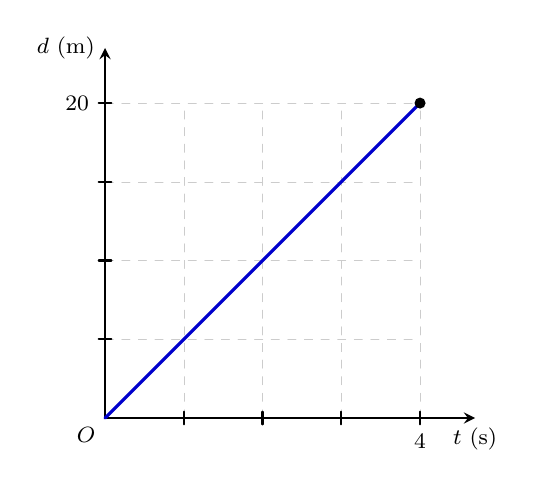
\begin{tikzpicture}[x=1cm, y=1cm, >=stealth, line join=round, line cap=round, font=\footnotesize]
	% 1. Lưới nền 4x4
	\draw[help lines, gray!40, dashed] (0,0) grid (4,4);
	
	% 2. Trục tọa độ
	\draw[->, thick] (0,0) -- (4.7,0) node[below] {$t\text{ (s)}$};
	\draw[->, thick] (0,0) -- (0,4.7) node[left] {$d\text{ (m)}$};
	\node[below left] at (0,0) {$O$};
	
	% 3. Vạch chia và số
	\foreach \x in {1,2,3,4} {
		\draw[thick] (\x, 0.08) -- (\x, -0.08);
	}
	\node[below] at (4, -0.08) {$4$};
	
	\foreach \y in {1,2,3,4} {
		\draw[thick] (0.08, \y) -- (-0.08, \y);
	}
	\node[left] at (-0.08, 4) {$20$};
	
	% 4. Đồ thị
	\draw[very thick, blue!80!black] (0,0) -- (4,4);
	\fill[black] (4,4) circle (2pt);
\end{tikzpicture}
\end{document}
